\chapter{Skill-biased technical change}\label{ch:2}

We begin our exploration of technical change by analzying a simple model of an economy with labor-augmenting technology, of the type proposed by \citet{Griliches1969}.

\section{Related Literature}

Most early treatments of technical change in the economic literature assume `technology' has a uniform impact across all types of production. For example, in {\em Principles}, Ricardo considers two types of innovations: landsaving innovations, that increase the output of every grade of land equiproportionally, and capital-and-labor saving innovations, that scale the output of capital and labor inputs evenly across the economy.

More recent examples of this type of technology are frequently found in the growth accounting literature. Consider, for example, the neoclassical model of growth, which views production through the lens of the neoclassical production function, a kind of black-box function that `converts' inputs of capital and labor into an output good, using technology. Most formulations of the production function include a `productivity' parameter, that governs the rate at which factors of production are converted into outputs. Solow's (\citeyear{Solow1957}) well-known functional form, $F(K,L,t)=A(t)f(K,L)$, included measures for capital ($K$) and labor ($L$) inputs, but also allowed `technology' ($A(t)$) to vary over time. He deliberately left the definition of technology vague, to simply mean any change in the rate of production: ``all sorts of things will appear as technical change'' \citep[p.312]{Solow1957}. 

In Solow's accounting scheme, technology could simply be computed as the `residual' between output and $f(K,L)$. In his 1957 paper, Solow employed US national accounting statistics for real GDP, capital and labor. Between 1909 and 1949, he estimated that total factor productivity increased more or less monotonically, and by 1949 $A$ had grown to about double its initial value. Taken together with Solow's (\citeyear{Solow1956}) model of long-run growth, one important use for Solow's contribution was to spur the field of growth accounting. This approach to studying income spawned a large empirical literature studying the causes of economic growth and development. Today, the neoclassical approach remains an important class of models in the study of the patterns of international income and growth. A prominent example is \citet{Mankiw1992}, which shows that the Solow model, augmented for a measure of human capital, explains cross-country variation in incomes very well indeed. The neoclassical growth model, as elegant and convenient as any economic model can be, was only successful explaining income differences between, and not within, countries.

\subsection{Explanations for Rising U.S. Education Premia}

By the 1980s, empirical evidence from the United States suggested that the rental rate of skilled workers had begun to grow considerably faster than that of unskilled workers \citep{Juhn1993}. Until then, wage growth differentials between different skill and educational groups had remained more or less stable. At the same time, the supply of skilled workers in the United States, relative to unskilled workers, had grown dramatically. The presence of a systematic difference in the wage rate of different types of workers implies that, since firms were willing to pay higher wage rates for skilled workers than unskilled workers, despite a relative increase in supply, suggests that the marginal productivity of skilled workers had grown to be higher than that of unskilled workers. Solow's simple but elegant model, which makes no distinction between different kinds of workers, she no light onto this trend. A more nuanced understanding of the impact of technology on workers' productivity was needed.

One set of explanations pointed to the changing nature of labor market institutions. \citet{Freeman1994}, for example, suggested that the about 50 per cent of the increase in the `white collar' premium paid to U.S. men could be explained by the decline in the unionization rate. It is widely understood that union bargaining activities result in a narrowing of wage dispersion between unionized workers. He argued that a decrease in the union rate resulted in a loss of worker bargaining power, and thus a decrease in wages. But since unions tend to cover mainly `blue-collar' occupations, then this trend should result in a widening gap between blue- and white-collar work. Yet other explanations for the growing premium paid to skilled workers include sociological factors, such as changes in norms associated with worker pay \citep{Mitchell1989}. Alternatively, the decline in the density of union workers may simply reflect broader economic trends: changes in the nature and distribution of production activity, for instance.

One economic trend that could bring about a change in the demand for skilled and unskilled labor is the transfer of many US manufacturing jobs overseas. This argument was advanced by \citet{Murphy1992}, who appeal to changes in the demand structure of US labor as a consequence of trade and competition with overseas producers. The patterns of U.S. trade shifted over the 1980s from trade surplus to deficits, favoring the manufacture of goods in low-cost countries, instead of with domestic, high-cost workers. \citename{Murphy1992} study the relationship between wage rates for white males between 1963 and 1979, and macroeconomic measures of output and wages both in the U.S. and overseas, concluding that changing patterns of trade go a long way to explain changes in the wage structure.

During this debate, some authors argued that technological progress might have softened demand for certain kinds of physical labor. Using logitudinal data gathered from census files, \citet{Davis1991} argue that, though capital investment in automated equipment and machinery, the manufacturing sector  replaced labor-intensive jobs with plant capital. Under this explanation, growing wage differentials between college-educated workers and high school graduates is a result of changes in the demand for labor, as the demand for non-manual work expands, and the demand for manual labor softens. \citet{Krueger1993} expands on this argument, and using microdata on individual workers, finds a premium associated with those occupations that involve computer use.\footnote{For a rather cynical refutation of Krueger's position, see \citet{DiNardo1997}, who show that an effect of a similar magnitude is associated with occupations that use pencils.}

\subsection{Models of Skill-Biased Technological Change}

The predominant explanation that came to be accepted in the literature is that new technologies, emerging over the post-war era, are complementary to skilled work. \citet{Tinbergen1974,Tinbergen1975} developed a model of the labor market where different kinds of labor were factors in production. Since the time of Adam Smith, it has been well known that the productivity of modern production processes, at any scale, depends crucially on the specialization of labor into a number of different jobs. In Adam Smith's famous study of a pin factory, Smith observed somewhere between a 240-- and 4800--factor increase because of complementarities between different, specialized jobs \citet[I.3]{Smith1776}. Tinbergen recognized that it would be unwieldy to attempt to model every of job using a production function, as the dimensionality of the model would quickly explode. However, armed with the observation that many properties of jobs are highly correlated, he proposed that a good characterization of the labour market can be made by singling out just one or two properties of different jobs. One particularly relevant property of jobs is the degree of {\em schooling} an individual has received. \citet{Tinbergen1974} modeled `graduate' and `unskilled' workers as imperfect substitutes in production, so that firms would seek to employ some number of both types of workers. 

Tinbergen identified two implications of his model. First, since the higher-productivity `graduate' workers were scarce relative to the supply of unskilled workers, graduates would be able to charge employers `scarcity rents,' as well as additional rents for their individual productivity. In the medium run, the availability of these rents would initiate a `race' for investment in education, as unskilled workers seek to enter education in order to access these rents.

Tinbergen's model was further developed by \citet{Katz1992} and others, and brought to bear on the empirical regularity of rising educational returns in the United States and elsewhere, beginning in the 1980s. In their model, they suggest that new workplace technologies disproportionately complement highly-skilled technical and managerial jobs, relative to low-skilled manual and service jobs. Under this explanation, the premium paid to high-skilled labor increases for two reasons: first, since high-skilled workers become relatively more productive, wages to high-skilled occupations are higher at the margin. There is also evidence that, in the United States at least, an increase in the demand for skilled labor, relative to its supply, has resulted in higher wages for skilled occupations. In the jargon, such technologies are said to exhibit \emph{skill bias} \citep{Autor2006}. 

One alternative to the canonical model of exogenous skill-biased technological change is presented by \citet{Beaudry2005}. They consider technical change as a discrete event, and model two `modes of production' as two separate production functions: the `old' and the `new.' In their model, the transition to the new technology is gradual, as capital of the old type is gradually replaced by the new. Importantly, their model implies that any inequality caused by the change in technology should eventually {\em narrow} as more capital is invested in the new technology, and the economy switches over to the new mode of production. At the point of the new technology's invention, only a small fraction of the economy is earning higher incomes by exploiting the new technology. But as the transition to the new type of technology completes, this difference should fade completely. Applied to skill-biased technology that exhibits capital-skill complementarity, this model implies that further investments in computer technology should actually {\em decrease} between-group inequality.

\subsection{Empirical Evidence for SBTC}

The empirical literature, which provides strong evidence for the SBTC thesis in foreign labor markets, has somewhat mixed support in Australia. Although there is a wealth of analysis on occupational change in the Australian labor market, less work has been done analyzing skill premia: largely this is because the patterns visible in the US and European labor markets are not present in the Australian context. However, many studies have confirmed a growing demand for skilled labor, as well as an associated growth in its supply.

The first group of studies look at changes in the workers' distribution of `skills'. The majority of these studies are demographic in nature, and tend provide descriptive statistics of changes in occupations as reported in sample surveys. Skill information is generally derived from occupational classification schemes.

The following group of studies examines 

Cover decomposition approach in more detail in Chapter~\ref{ch:4}.

The theory of skill-biased technical change with skill-capital complementarity outlined above suggests that two regularities should be observed in the data. First, 

\subsubsection{Upskilling in Australia}

Starting in the 1980s, in the United States a divergence between the rental rates of skilled an unskilled labor began to emerge. \citet{Acemoglu2011} report that the `skill premium' paid to college-educated workers remained relatively steady between 1964 and 1980, oscillating in the range of between 48 and 58 per cent, holding other factors constant. However, from 1980, this premium increased steadily 

We will take as a point of departure the standard model for analyzing skill-based technical change (SBTC). This model, dubbed the `canonical' model by \citet{Acemoglu2011} and which has sparked a voluminous literature, has enjoyed considerable empirical success explaining rising wages for high-skill managerial and professional jobs in the United States and Europe \citep{Katz1992}. Since the canonical model includes \emph{factor-augmenting} capital, it predicts a uniform skill upgrading of the work force at all education levels \citep{Levy2003}. Skill upgrading has been confirmed by a number of authors, both in Australia \citep{Esposto2012, Wooden2000, Cully1999} and overseas \citep{Autor2008}. 

Australian labor market definitely increasing in (1) skills, (2) knowledge intensity. \citet{Esposto2012} \citet{Esposto2011}

\cite{Cully1999} % upskilling, but no skill bias for Australia

\cite{Barnes2002} % 1990s, skilled empt incr 3% py ... see p. XI

\cite{Wooden2000} % upskilling and some evidence of skill polarisation. consistent with international evidence

\cite{Card2001} % supply <-> college premium

\cite{Borland1999}
\cite{Borland2000}

\subsubsection{The Skill Premium}

Direct studies of occupations have found that technology use within a job does indeed carry a skill premium. \citet{Borland2004} 

\cite{Autor1998} % computers <-> labor market

\cite{Coelli2009}

\section{Model}

The formulation of the SBTC model that gained wide acceptance in the literature, dubbed the `canonical model' by \citet{Acemoglu2011},  was deployed by a large number of authors analyzing skill-biased technology \citep[e.g.]{Katz1992,Goldin2007}. % etc
Before discussing the empirical evidence for SBTC, we will briefly outline the main features and implications of this model, following the notation employed by \citet{Acemoglu2011}

Consider a competitive economy with two different, imperfectly substitutable types of labor: high-skilled and low-skilled. Workers are heterogeneous, with different levels of efficiency within each skill group. Let the total supply of high-skilled labor be $H$, and the total supply of low-skilled labor be $L$, and both types are paid the same wage, respectively $w_h$ and $w_\ell$. Production in this economy is governed by a CES aggregate production function, with elasticity of substitution $\sigma$, where $\sigma>1$:
\begin{equation}  \label{eq:prod}
Y = \left[
  \left(A_LL \right)^\frac{\sigma-1}{\sigma}
  +
  \left(A_HH \right)^\frac{\sigma-1}{\sigma}
  \right]^\frac{1}{\sigma-1}.
\end{equation}

For our purposes, we are interested in two claims about relative wages made by this model: first, that technological change or a generalized shift from low-skilled to high-skilled work should never cause low-skilled wages to decrease, and second, that technological change should result in a monotonic increase in wage across the skill spectrum. To see this, we will first derive the expressions for the equilibrium wage for each type of labor. Since the economy is competitive, unique equilibrium wages for both both high- and low-skilled workers are given by their respective marginal products. Wages can therefore be found by differentiating \eqref{eq:prod} with respect to labor supply:
\begin{align}
w_h &= \frac{\partial Y}{\partial H} 
     = A_H^\frac{\sigma-1}{\sigma}\left(
              A_L^{\frac{\sigma-1}{\sigma}} (H/L)^{-\frac{\sigma-1}{\sigma}} + A_H^{\frac{\sigma-1}{\sigma}}
        \right)^{\frac{1}{\sigma - 1}} \label{eq:wh} \\
w_l &= \frac{\partial Y}{\partial H} 
     = A_L^\frac{\sigma-1}{\sigma}\left(
              A_L^{\frac{\sigma-1}{\sigma}} + A_H^{\frac{\sigma-1}{\sigma}}(H/L)^{\frac{\sigma-1}{\sigma}}
        \right)^{\frac{1}{\sigma - 1}} \label{eq:wl}
\end{align}
The first claim follows from differentiating these wage equations. First, notice in \eqref{eq:wl} that $\partial w_L/\partial A_H \geq 0$. This means that, in this model, an increase in technology for high-skilled workers does not reduce the wage for low-skilled workers. Technological progress should in fact result in positive wage improvements for both high- and low-skilled workers. 

Next, notice that $\partial w_l/\partial(H/L)>0$. An increase in the relative supply of high-skilled workers, $H/L$, should therefore not decrease the wage of low-skilled workers. Rather, as high-skilled work becomes more productive and the ratio of skilled to unskilled workers increases, the demand for low-skilled work simultaneously increases. 

Second, consider the ratio between high- and low-skilled labor, $\omega=w_h/w_l$ (for convenience, we will consider the log ratio.) It is straightforward to show that this ratio depends on the state of technology and labor inputs:
\begin{equation}\label{eq:omega}
\log \omega = \frac{\sigma-1}{\sigma}\log\left(\frac{A_H}{A_L}\right) - \frac{1}{\sigma}\log\left(\frac{H}{L}\right).
\end{equation}
This equation illustrates the two countervailing forces of Tinbergen's (1974) `race' for education that govern the magnitude of the skill premium. Holding the labor supply ratio constant, and recalling our assumption that $\sigma >1$, an increase in skill-biased technology $A_H/A_L$ results in a larger $\log\omega$. On the other hand, holding technology constant, an increase in the proportion of workers providing high-skilled labor should decrease the log skill premium.\footnote{Formally, $\partial \log\omega / \partial(A_H/A_L) > 0$, and 
$\partial \log\omega / \partial(H/L) < 0$.} In this model, a rising skill premium occurs when the first term of \eqref{eq:omega}  dominates the second.

To review, the SBTC model claims that unless there is technical regress, wages for all skill types will always increase, and never decrease (wages should follow a monotonic path.) Second, in the presence of an increasing proportion of workers conducting skilled work, the model is consistent with either a rising or a falling log skill premium.

\section{Data}

To bring the SBTC model to the data, we employ the Survey of Income and Housing, a hierarchical clustered household survey conducted by the ABS every 2-3 years since 1995, and also for the fiscal years 1985-6 and 1981-2. The survey provides detailed  information about respondents' labor and non-labor income sources, as well as data on age, educational attainment, hours worked and industry and occupation. For the surveys conducted between 2000 and 2010, as well as the 1981-2 survey, the data include detailed occupational data, which will become important later. The other surveys include occupation only at the one-digit level. We obtain survey micro-data as confidentialized unit record files (CURFs).

To facilitate inter-temporal comparisons, we must eliminate effects which arise as a result of mechanical, demographic shifts. Between 1982 and 2010, the number of women in the work force has increased dramatically, and the same period has seen an evolution of the educational and age composition of the work force, and the rate of casual and part-time employment has increased. Following \citet{Acemoglu2011}, we therefore include only full-time workers for whom labor forms the primary source of income. We further composition-adjust each survey to match 2010 demographics by linearly scaling the survey selection weights for each age group/sex/educational group cell. All computations in this study treat these adjusted weights as inverse selection probabilities.

\begin{figure}
  \centering
  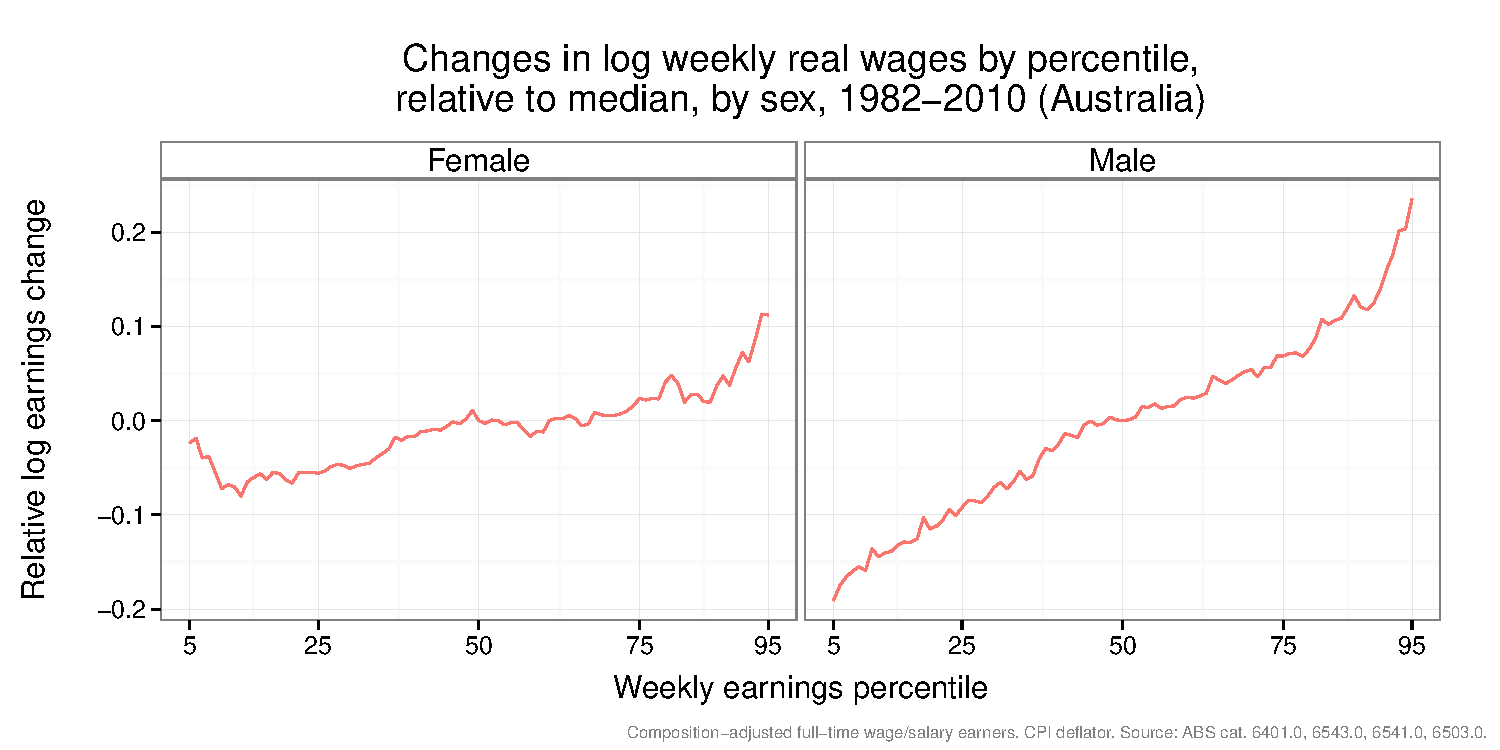
\includegraphics[width=\textwidth]{../figure/quantile_mf.pdf}
  \caption{Change in weekly wage by percentile, 1981-2010, Males and Females. Full-time workers whose main sources of income are wages and salaries are shown. Notice that real wage growth has been non-monotone for males in lower percentiles. Source: Survey of Income and Housing.}
  \label{fig:banana}
\end{figure}

\section{Results}

If SBTC explained the widening of the income distribution, we would expect to observe the premium accruing to `skilled' labor increasing with time. Figure~\ref{fig:banana} shows the composition-adjusted changes in log real wage by percentile, for males and females, between 1981-82 and 2009-10. If the 1981-82 income percentile can be considered a proxy for skill, then it is apparent that, over this period, wages more grew for high-skill individuals much faster than for low-skill individuals. It would therefore be expected that the premium accruing to higher educational attainment would show a similar trend.

In the United States, at least, the wage premium earned by tertiary-educated labor fell in the 1970s, but has risen each decade since then \citep{Acemoglu2011}. \citet{Katz1992} employs a similar empirical model which explains the rise of the skill premium in the United States in the post-war era. In Australia, however, a corresponding growth in the premium for tertiary qualifications has not been observed. Figure~\ref{fig:wagepremium} shows the log skill premium for Australia and the United States between 1982 and 2008. Rather than any fundamental differences in the nature of the demand for skills, \citet{Coelli2009} attributes this difference in Australian workers to differences in the nature of Australian educational qualifications. In Australia, University degrees are available to a wider range of candidates and for a wider range of disciplines than those who would traditionally have undertaken university studies in the United States. As a result, tertiary educational attainment may be a poor proxy for `skilled' work in Australia.
\begin{figure}
  \centering
  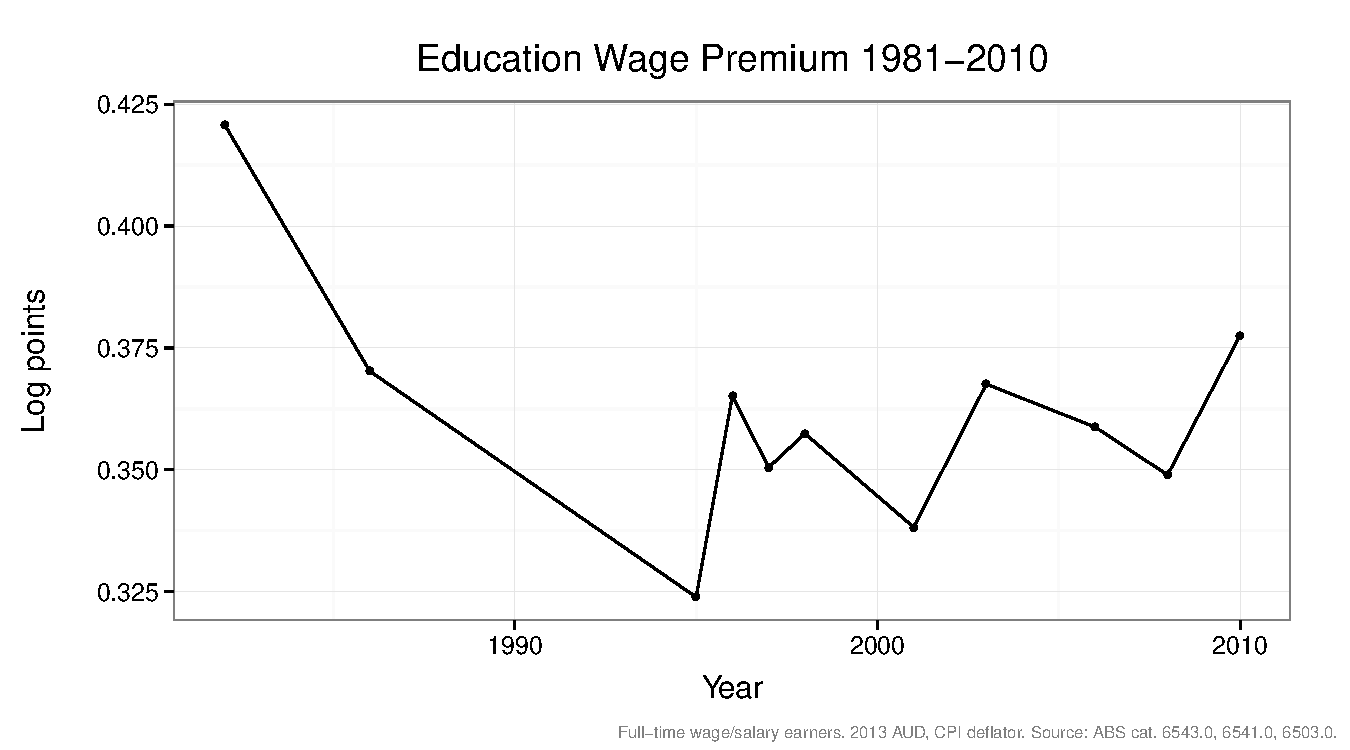
\includegraphics[width=\textwidth]{../figure/ed_premium_time_two.pdf}
  \caption{University/non-university log wage premium, Australia and the United States. The figures show the difference between the mean log weekly income for workers who have attained a bachelor degree or higher, and the mean weekly income of other workers. Only full-time workers whose main sources of income are wages and salaries are included, and survey data have been composition adjusted for sex, age group, (and for the United States, race). Source: for Australia, ABS Survey of Income and Housing, and for the United States, \citet{Acemoglu2011}.}
  \label{fig:wagepremium}
\end{figure}

The SBTC model also claims that, even if technology exhibits skill bias, wages for all skill groups should increase monotonically. Figure~\ref{fig:changetime} plots the cumulative change over time for three wage percentiles, the 5th, 95th, and the median. Over the period 1981-82 to 2009-10, although wages at the top percentiles increased steadily, the same is not true for the lower percentiles. Indeed, for all of the 1990s and much of the 2000s, cumulative real income growth from 1981-82 was negative for many workers.
\begin{figure}
  \centering
  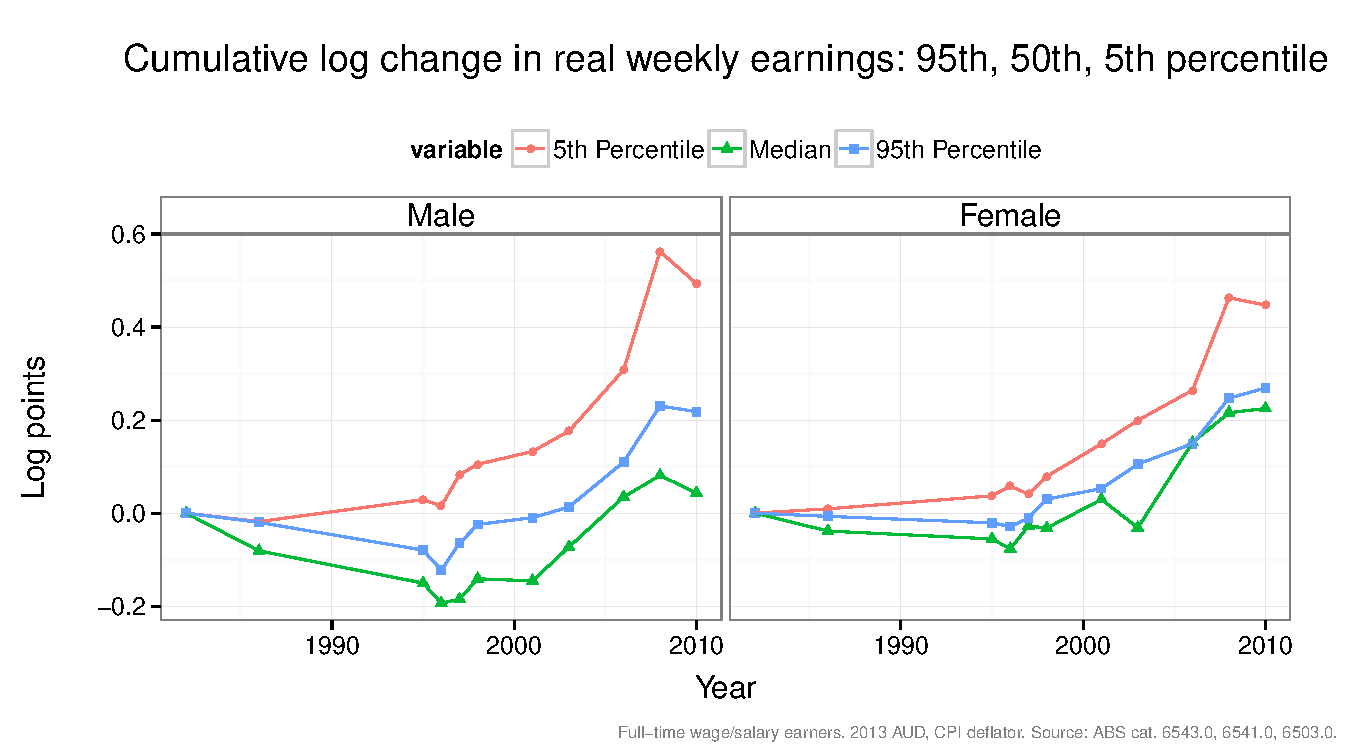
\includegraphics[width=\textwidth]{../figure/wage_change_time.pdf}
  \caption{Cumulative log change in real weekly earnings, 5th, 50th and 95th percentiles, 1982-2010. Full-time workers whose main sources of income are wages and salaries are shown. Notice that real wage growth has been non-monotone for males in lower percentiles. Source: Survey of Income and Housing.}
  \label{fig:changetime}
\end{figure}

\section{Conclusion}

That the income distribution is widening, but the skill premium is {\em not} driving the change, suggests one of at least two interpretations. We have already discussed the fact that educational attainment may be a poor indicator of skill for the Australian labor market. A second, more nuanced explanation was given by \citet{Levy2003}. Technological change may not be complementary to all types of labor; it may replace many types of labor entirely.





%%% Local Variables: 
%%% mode: latex
%%% TeX-master: "thesis"
%%% End: 
